\documentclass[border=4pt]{standalone}
\usepackage[utf8]{inputenc}
\usepackage[T1]{fontenc}
\usepackage{amsmath,amssymb}
\usepackage{tikz}
\usetikzlibrary{arrows.meta,positioning,calc}
\usepackage{pgfplots}
\pgfplotsset{compat=1.18}
\newcommand{\vect}[1]{\mathbf{#1}}
% Se compila desde la carpeta docs/: las rutas de datos son relativas a ella.
\begin{document}
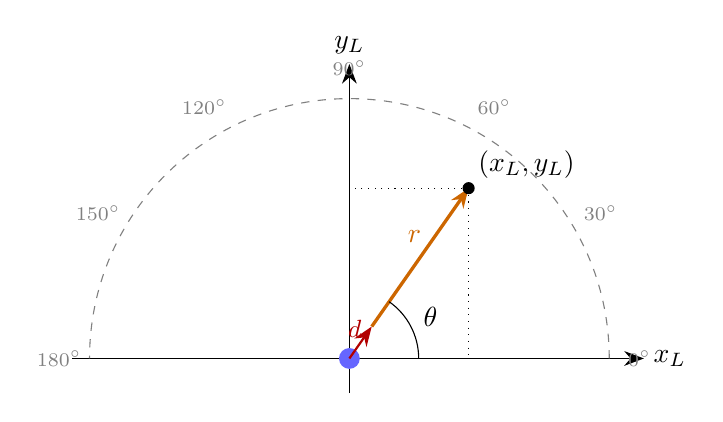
\begin{tikzpicture}[scale=1.1, >={Stealth[length=2.5mm]}]
\draw[->] (-3.2,0) -- (3.4,0) node[right] {$x_L$};
\draw[->] (0,-0.4) -- (0,3.4) node[above] {$y_L$};
\draw[dashed, gray] (3,0) arc (0:180:3);
\foreach \a in {0,30,...,180} \node[gray, font=\scriptsize] at (\a:3.35) {$\a^\circ$};
\fill[blue!60] (0,0) circle (0.12);
\draw[thick, red!70!black, ->] (0,0) -- (55:0.45);
\draw[very thick, orange!80!black, ->] (55:0.45) -- (55:2.4);
\fill (55:2.4) circle (0.07) node[above right] {$(x_L, y_L)$};
\draw (0.8,0) arc (0:55:0.8);
\node at (27:1.05) {$\theta$};
\node[red!70!black, font=\small] at (80:0.35) {$d$};
\node[orange!80!black] at (62:1.6) {$r$};
\draw[dotted] (55:2.4) -- ({2.4*cos(55)},0);
\draw[dotted] (55:2.4) -- (0,{2.4*sin(55)});
\end{tikzpicture}
\end{document}
